\appendix

\section{Declaración preliminar de uso de inteligencia artificial}
\begin{table}[H]
\centering
\small
\caption{Declaración de uso de herramientas de inteligencia artificial.}
\begin{tabularx}{\textwidth}{L{3.5cm}Y}
\toprule
\textbf{Campo} & \textbf{Declaración del equipo} \\
\midrule
Herramienta y versión & ChatGPT (OpenAI) y Claude (Anthropic); versión o modelo no especificado. \\
Propósito & Apoyo en la estructuración y organización de información, redacción y revisión ortográfica del contenido. En el segundo corte, además, apoyo en la revisión de la consistencia técnica entre secciones. \\
Secciones apoyadas & Organización y redacción de apartados del informe, síntesis de información técnica y revisión de textos. En el segundo corte: actualización de las secciones de planeación, montaje físico, conclusiones y anexos. \\
Verificación realizada & La información sugerida fue analizada por el equipo y contrastada con fuentes externas confiables, incluyendo páginas oficiales de fabricantes y fichas técnicas consultadas para elaborar la caracterización de los equipos. Los datos técnicos del segundo corte (datos de placa, mediciones, resultados del ensayo y parámetros del controlador) provienen del prototipo y de los integrantes del equipo; la inteligencia artificial no generó datos experimentales. \\
Responsabilidad & Los autores revisaron el contenido y asumen responsabilidad por su exactitud. \\
\bottomrule
\end{tabularx}
\end{table}

\section{Reporte de similitud}


\section{Evidencia del artículo en inglés}
Como evidencia del desarrollo del artículo científico, se adjunta la versión en inglés elaborada hasta la sección de Materials and Methods.

%\includepdf[pages=-]{articuloingles.pdf}

\section{Anexos técnicos}
\begin{itemize}
\item Anexo A: matriz QFD completa.
\begin{figure}[H] \centering \includegraphics[width=0.4\textwidth]{figuras/MATRIZ_QFD.png} \end{figure}
\item Anexo B: matrices Pugh completas.
Las matrices se encuentran ya cargadas dentro del documento para mejor comprensión lineal del proyecto
\item Anexo D: cálculos y simulaciones.

Los parámetros del modelo térmico de primer orden se obtienen a partir del
coeficiente global de pérdidas térmicas $UA$, la masa activa de fluido y el
calor específico del agua. Estos parámetros corresponden al modelo del
proceso y no a los parámetros de sintonía del controlador.

El valor de la ganancia estática del proceso se calcula como:

\begin{equation}
K = \frac{1}{UA}
= \frac{1}{4}
= 0{,}25\ \mathrm{K/W}
\end{equation}

La constante de tiempo del proceso se determina mediante:

\begin{equation}
\tau = \frac{m\,c_p}{UA}
= \frac{20 \times 4186}{4}
= 20\,930\ \mathrm{s}
\approx 348{,}8\ \mathrm{min}
\end{equation}

Por tanto, el modelo de primer orden utilizado para representar la dinámica
térmica del sistema queda definido por:

\begin{equation}
\boxed{
G(s) = \frac{0{,}25}{20\,930\,s + 1}
}
\end{equation}

En consecuencia, los principales parámetros obtenidos para el modelo son:

\begin{equation}
\boxed{
K=0{,}25\ \mathrm{K/W},
\qquad
\tau=20\,930\ \mathrm{s}\approx348{,}8\ \mathrm{min}
}
\end{equation}

\paragraph{Enlace al script de la simulación en lazo abierto}

El script utilizado para realizar la simulación en lazo abierto se encuentra
disponible en el siguiente enlace:

\begin{center}
\href{https://mailustabucaedu-my.sharepoint.com/:u:/g/personal/fabianaugusto_ruiz_ustabuca_edu_co/IQA-BS2GA_CMQ4VUrsyvaq6EAYTtpR_JWi9h-BOVhUr7l5k?e=7DXsHx}
{\textbf{Script de simulación en lazo abierto}}
\end{center}


\item Anexo F: evidencia del repositorio y del MOOC institucional.
\item Anexo G: información IP del PLC (primer corte; en el segundo corte se usó la dirección del Anexo~\ref{anx:programa_plc})
\begin{figure}[H] \centering 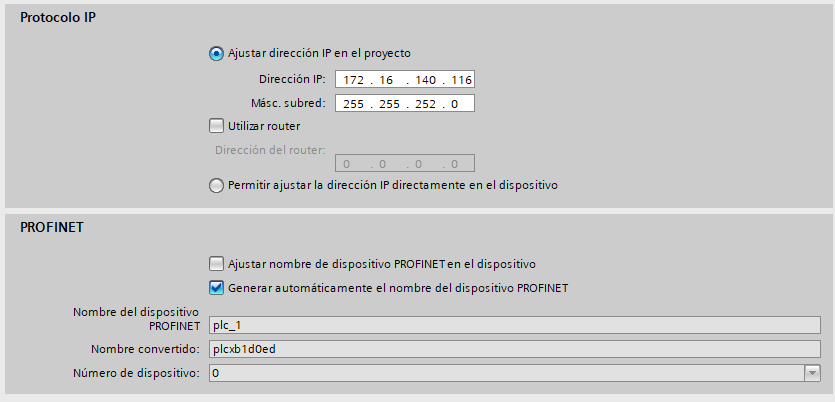
\includegraphics[width=0.4\textwidth]{figuras/DATOSPLC.png} \end{figure}
\item Anexo H: información IP del HMI (primer corte)
\begin{figure}[H] \centering 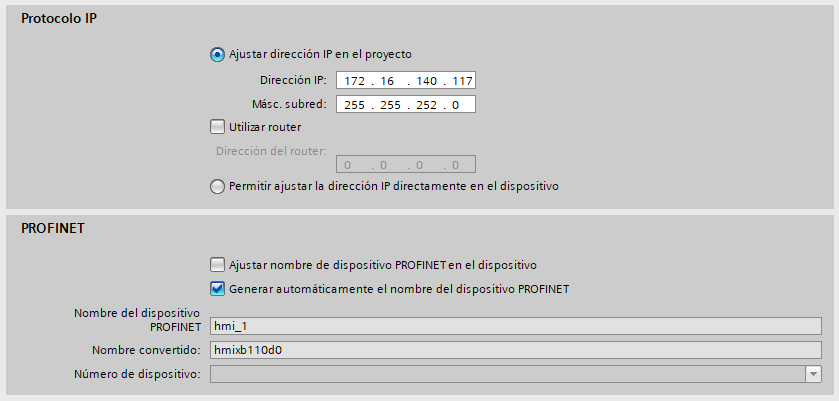
\includegraphics[width=0.4\textwidth]{figuras/DATOSHMI.png} \end{figure}
\item Anexo I: información IP del PC (primer corte)
\begin{figure}[H] \centering \includegraphics[width=0.5\textwidth]{figuras/IPPC.png} \end{figure}
\item \etiquetaanexo{J}{anx:programa_plc}Anexo J: programas del PLC (segundo corte). Se incluyen, como evidencia, las impresiones de TIA Portal de los dos programas descritos en la Sección~\ref{sec:montaje_programacion}:
\begin{itemize}
\item J.1: programa de la secuencia del ciclo CIP, bloque principal OB1 (Ladder v1.2).
\item J.2: programa de control de temperatura, interrupción cíclica OB30.
\item J.3: programa de control, bloque principal OB1 (registro de datos con \texttt{DataLog}).
\item J.4: bloque de datos \texttt{EXP} (DB1), variables del control y del ensayo.
\item J.5: bloque de datos \texttt{Datalog} (DB2), estructura del registro.
\item J.6: configuración del controlador \texttt{PID\_Compact\_1} (DB4).
\item J.7: tabla de variables del PLC del programa de control.
\item J.8: tabla de observación usada en el ensayo.
\item J.9: página \textit{Data logs} del servidor web del PLC, con los registros de los ensayos.
\end{itemize}
\end{itemize}

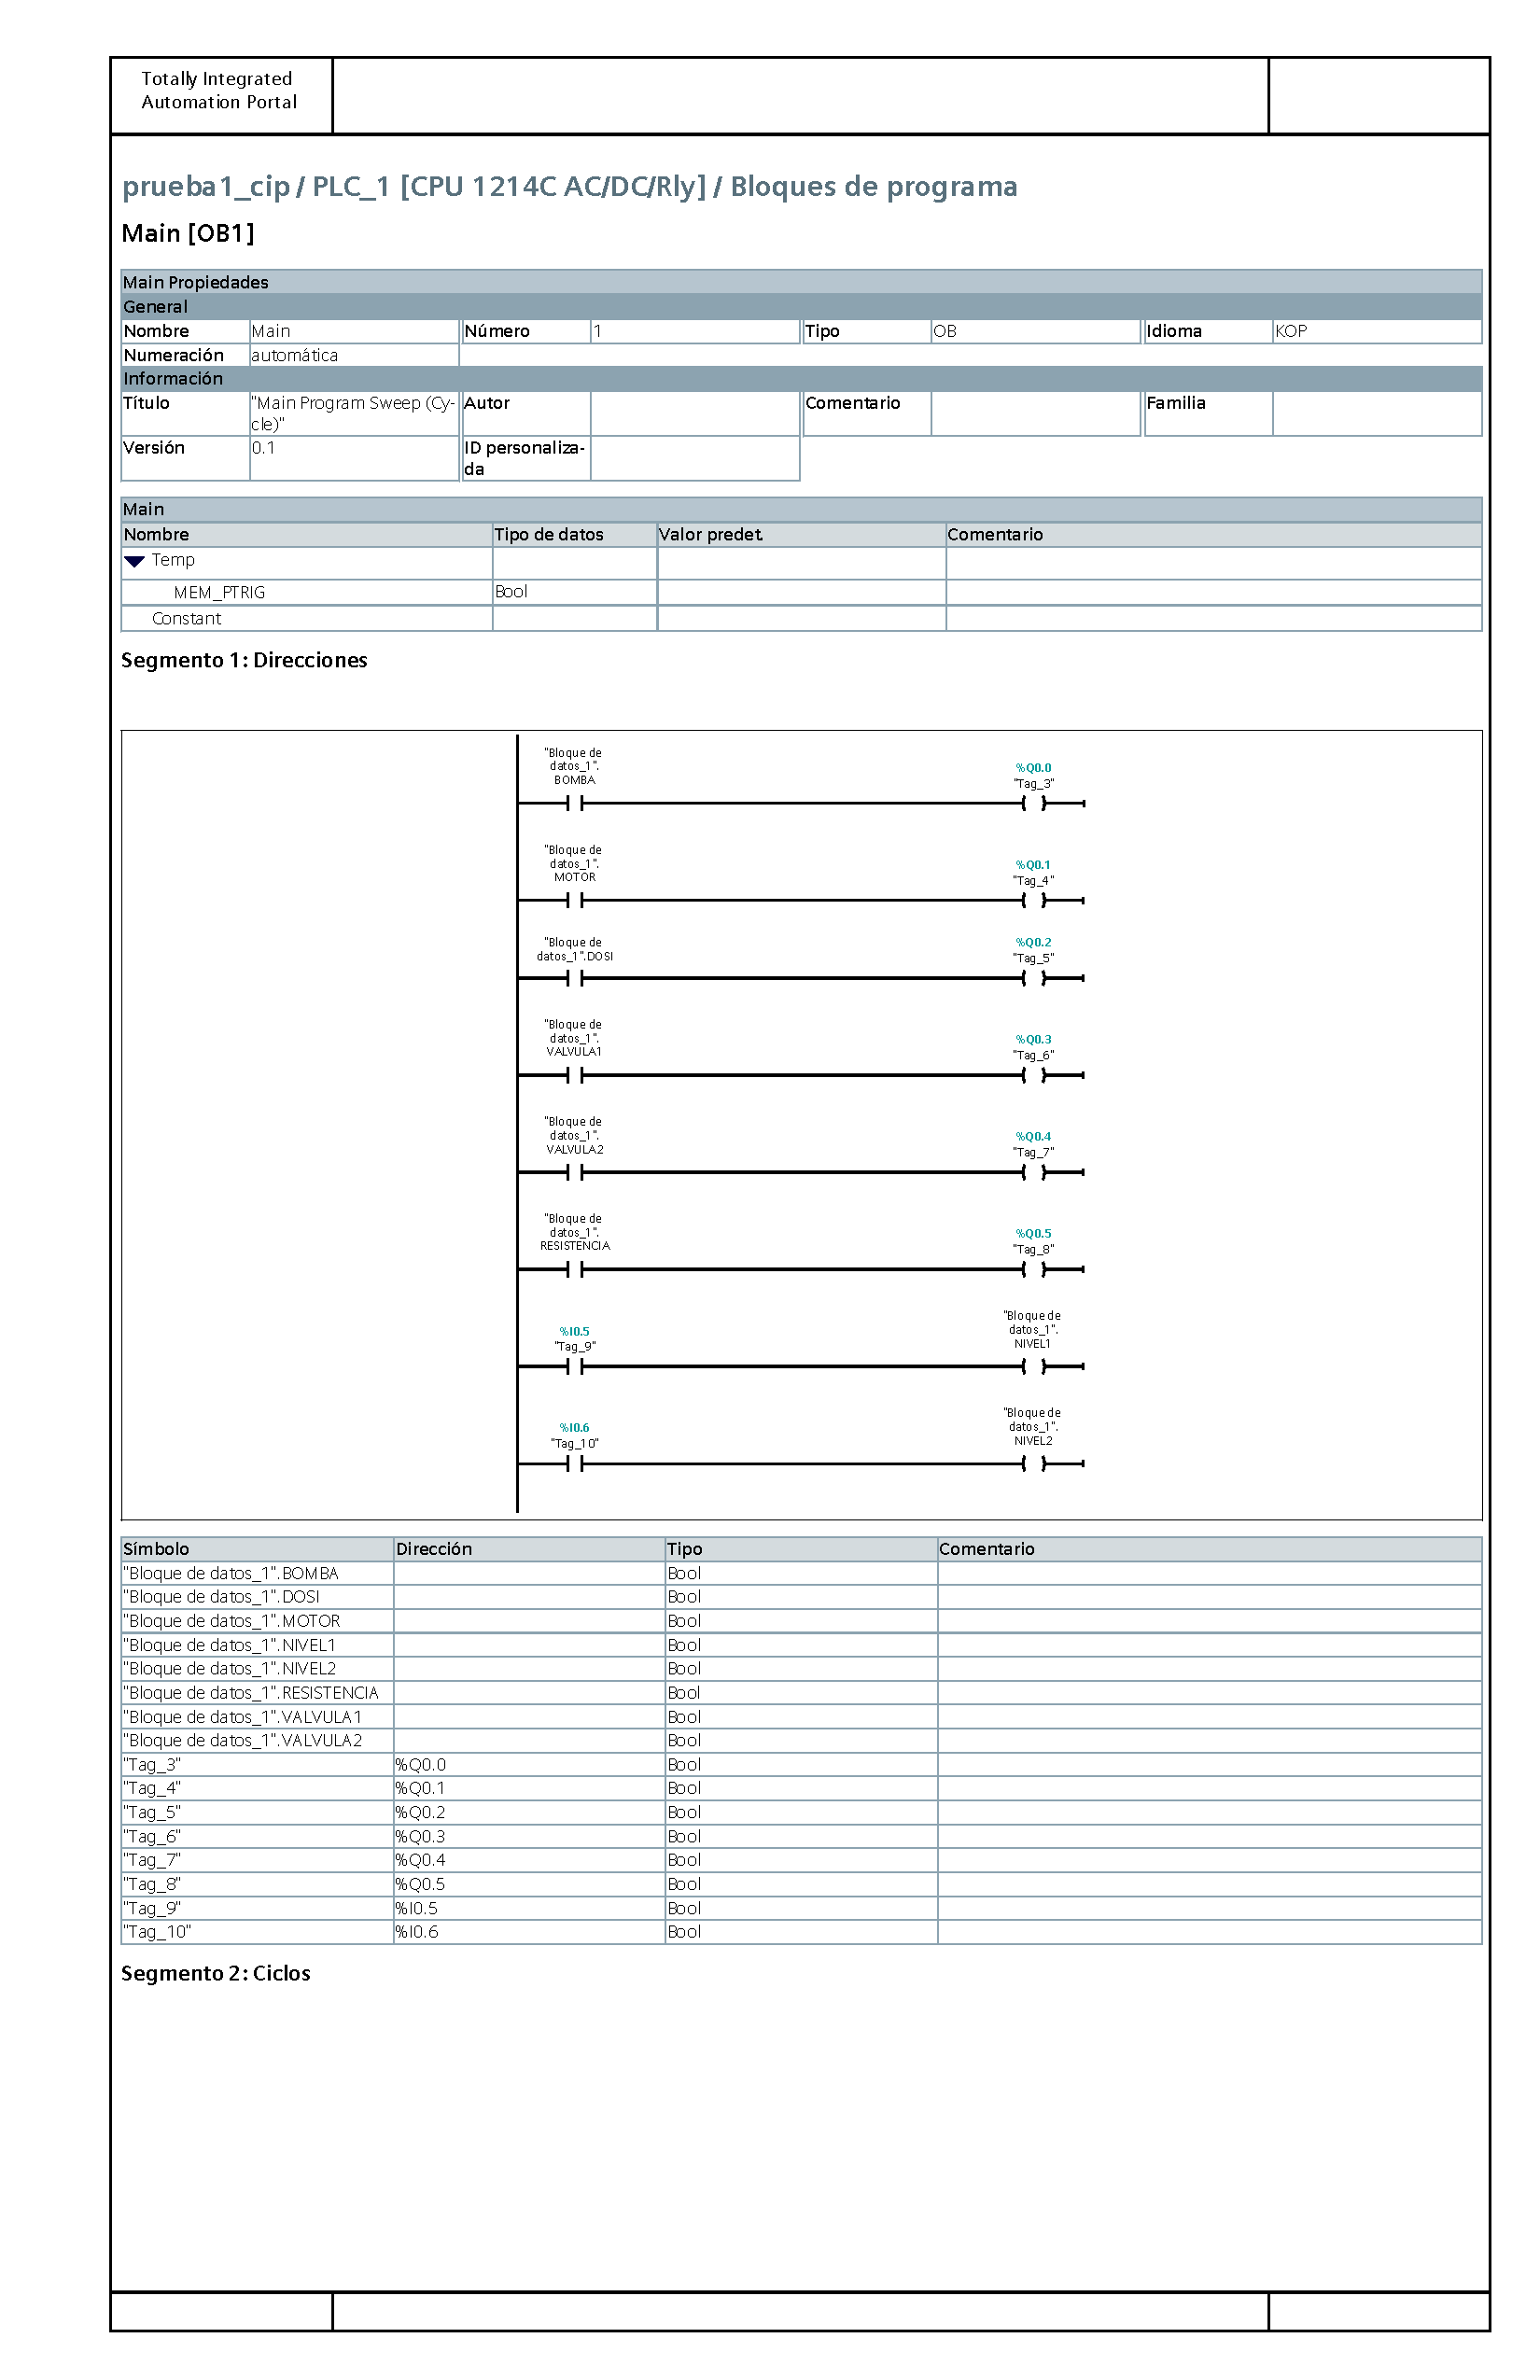
\includepdf[pages=1,scale=0.8,offset=0 -0.7cm,pagecommand={\thispagestyle{fancy}\noindent\textbf{J.1 Programa de la secuencia (OB1, Ladder v1.2)}}]{anexos/programa_plc/secuencia_OB1_ladder_v1_2.pdf}
\includepdf[pages=2-,scale=0.8,offset=0 -0.7cm,pagecommand={\thispagestyle{fancy}}]{anexos/programa_plc/secuencia_OB1_ladder_v1_2.pdf}
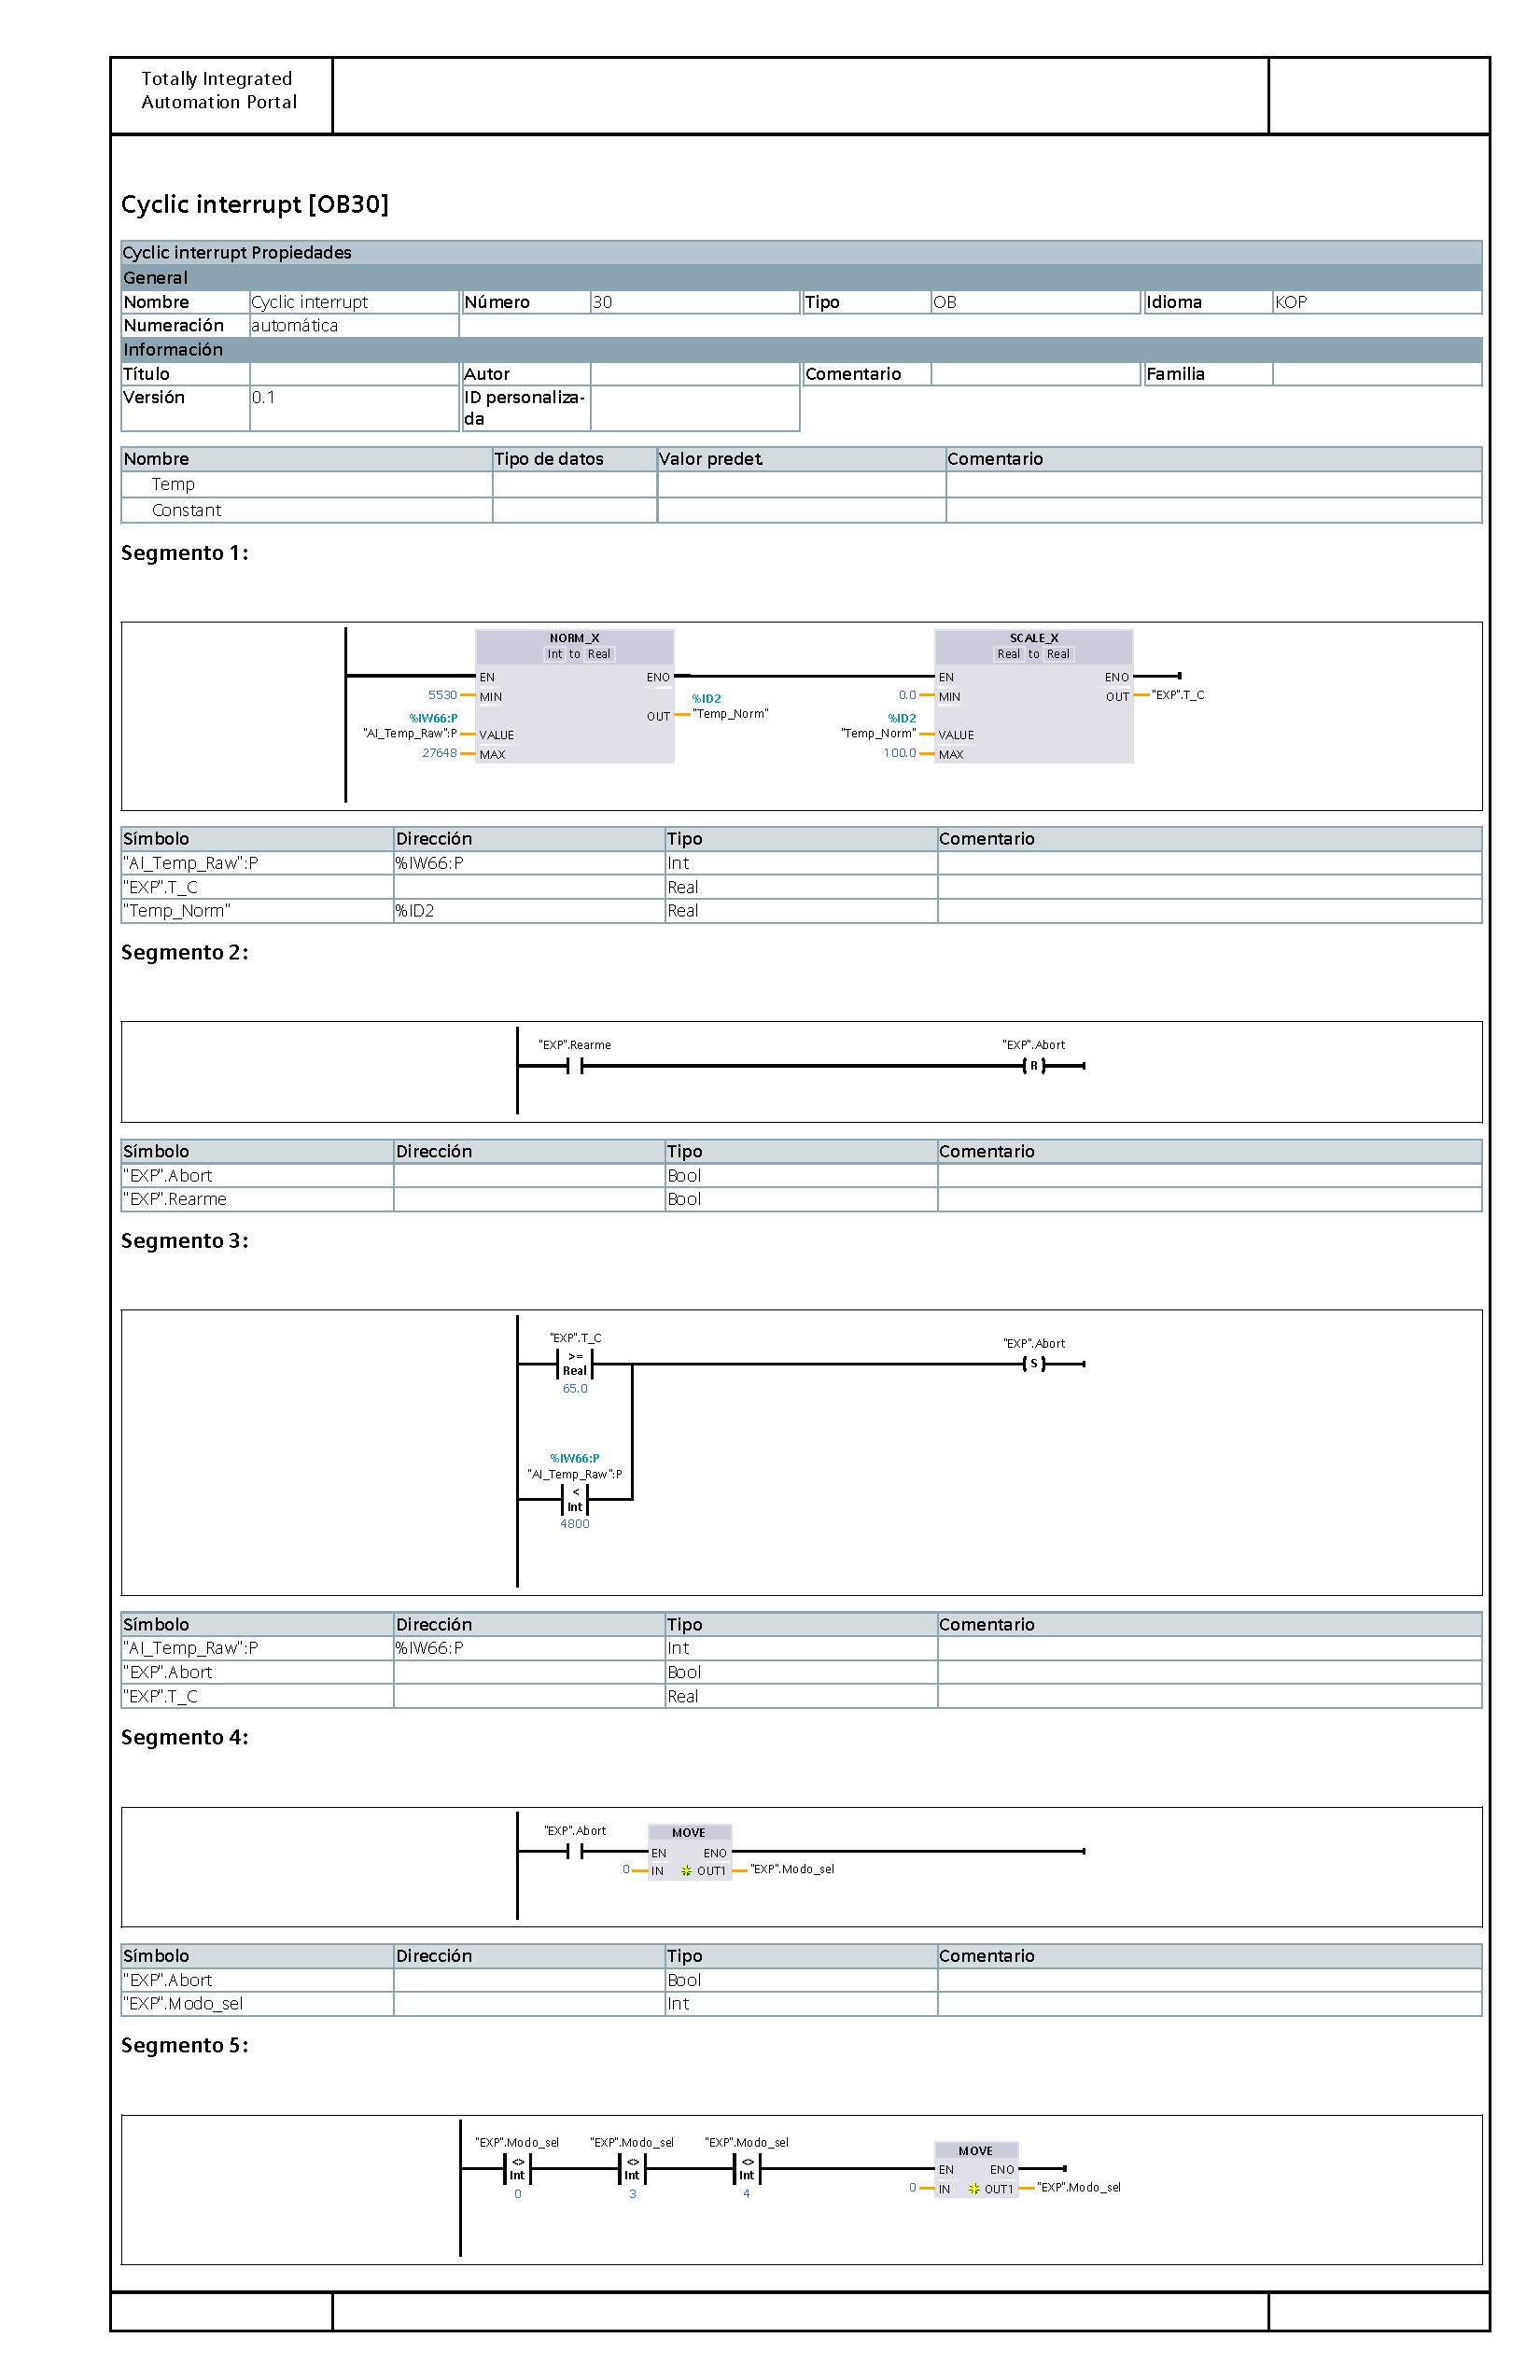
\includepdf[pages=1,scale=0.8,offset=0 -0.7cm,pagecommand={\thispagestyle{fancy}\noindent\textbf{J.2 Programa de control: interrupción cíclica (OB30)}}]{anexos/programa_plc/control_OB30_cyclic_interrupt.pdf}
\includepdf[pages=2-,scale=0.8,offset=0 -0.7cm,pagecommand={\thispagestyle{fancy}}]{anexos/programa_plc/control_OB30_cyclic_interrupt.pdf}
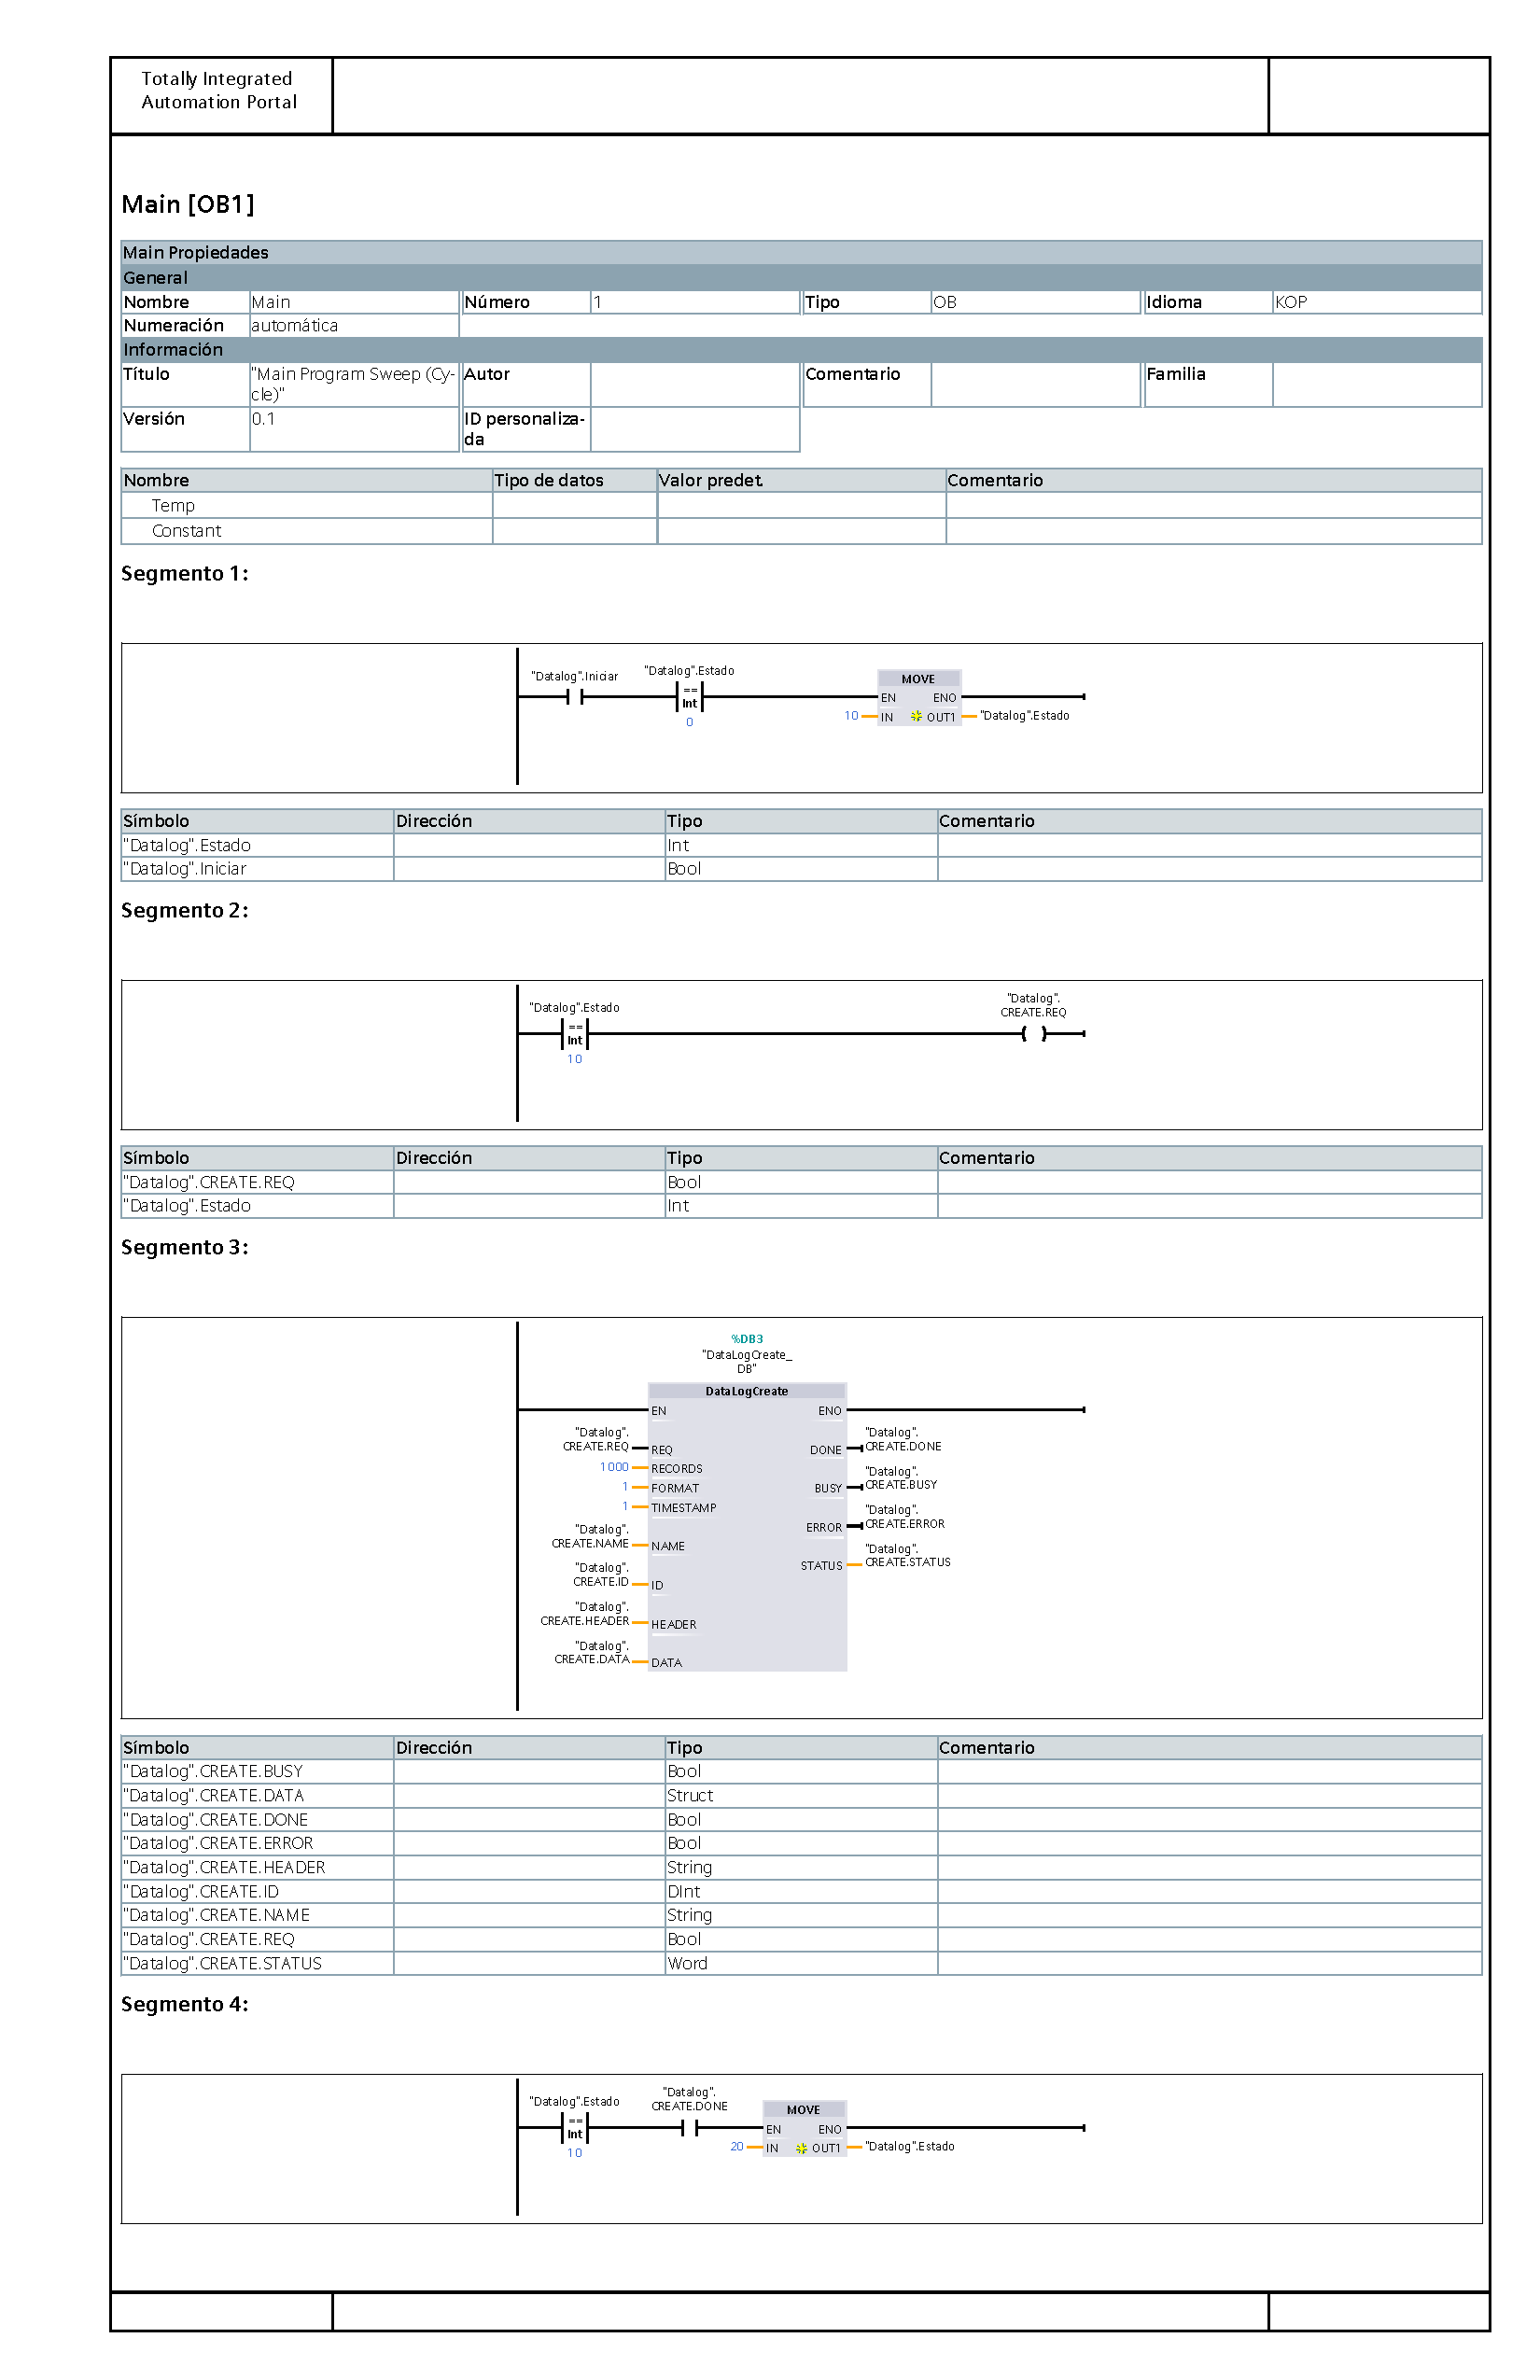
\includepdf[pages=1,scale=0.8,offset=0 -0.7cm,pagecommand={\thispagestyle{fancy}\noindent\textbf{J.3 Programa de control: bloque principal (OB1, registro de datos)}}]{anexos/programa_plc/control_OB1_main_datalog.pdf}
\includepdf[pages=2-,scale=0.8,offset=0 -0.7cm,pagecommand={\thispagestyle{fancy}}]{anexos/programa_plc/control_OB1_main_datalog.pdf}
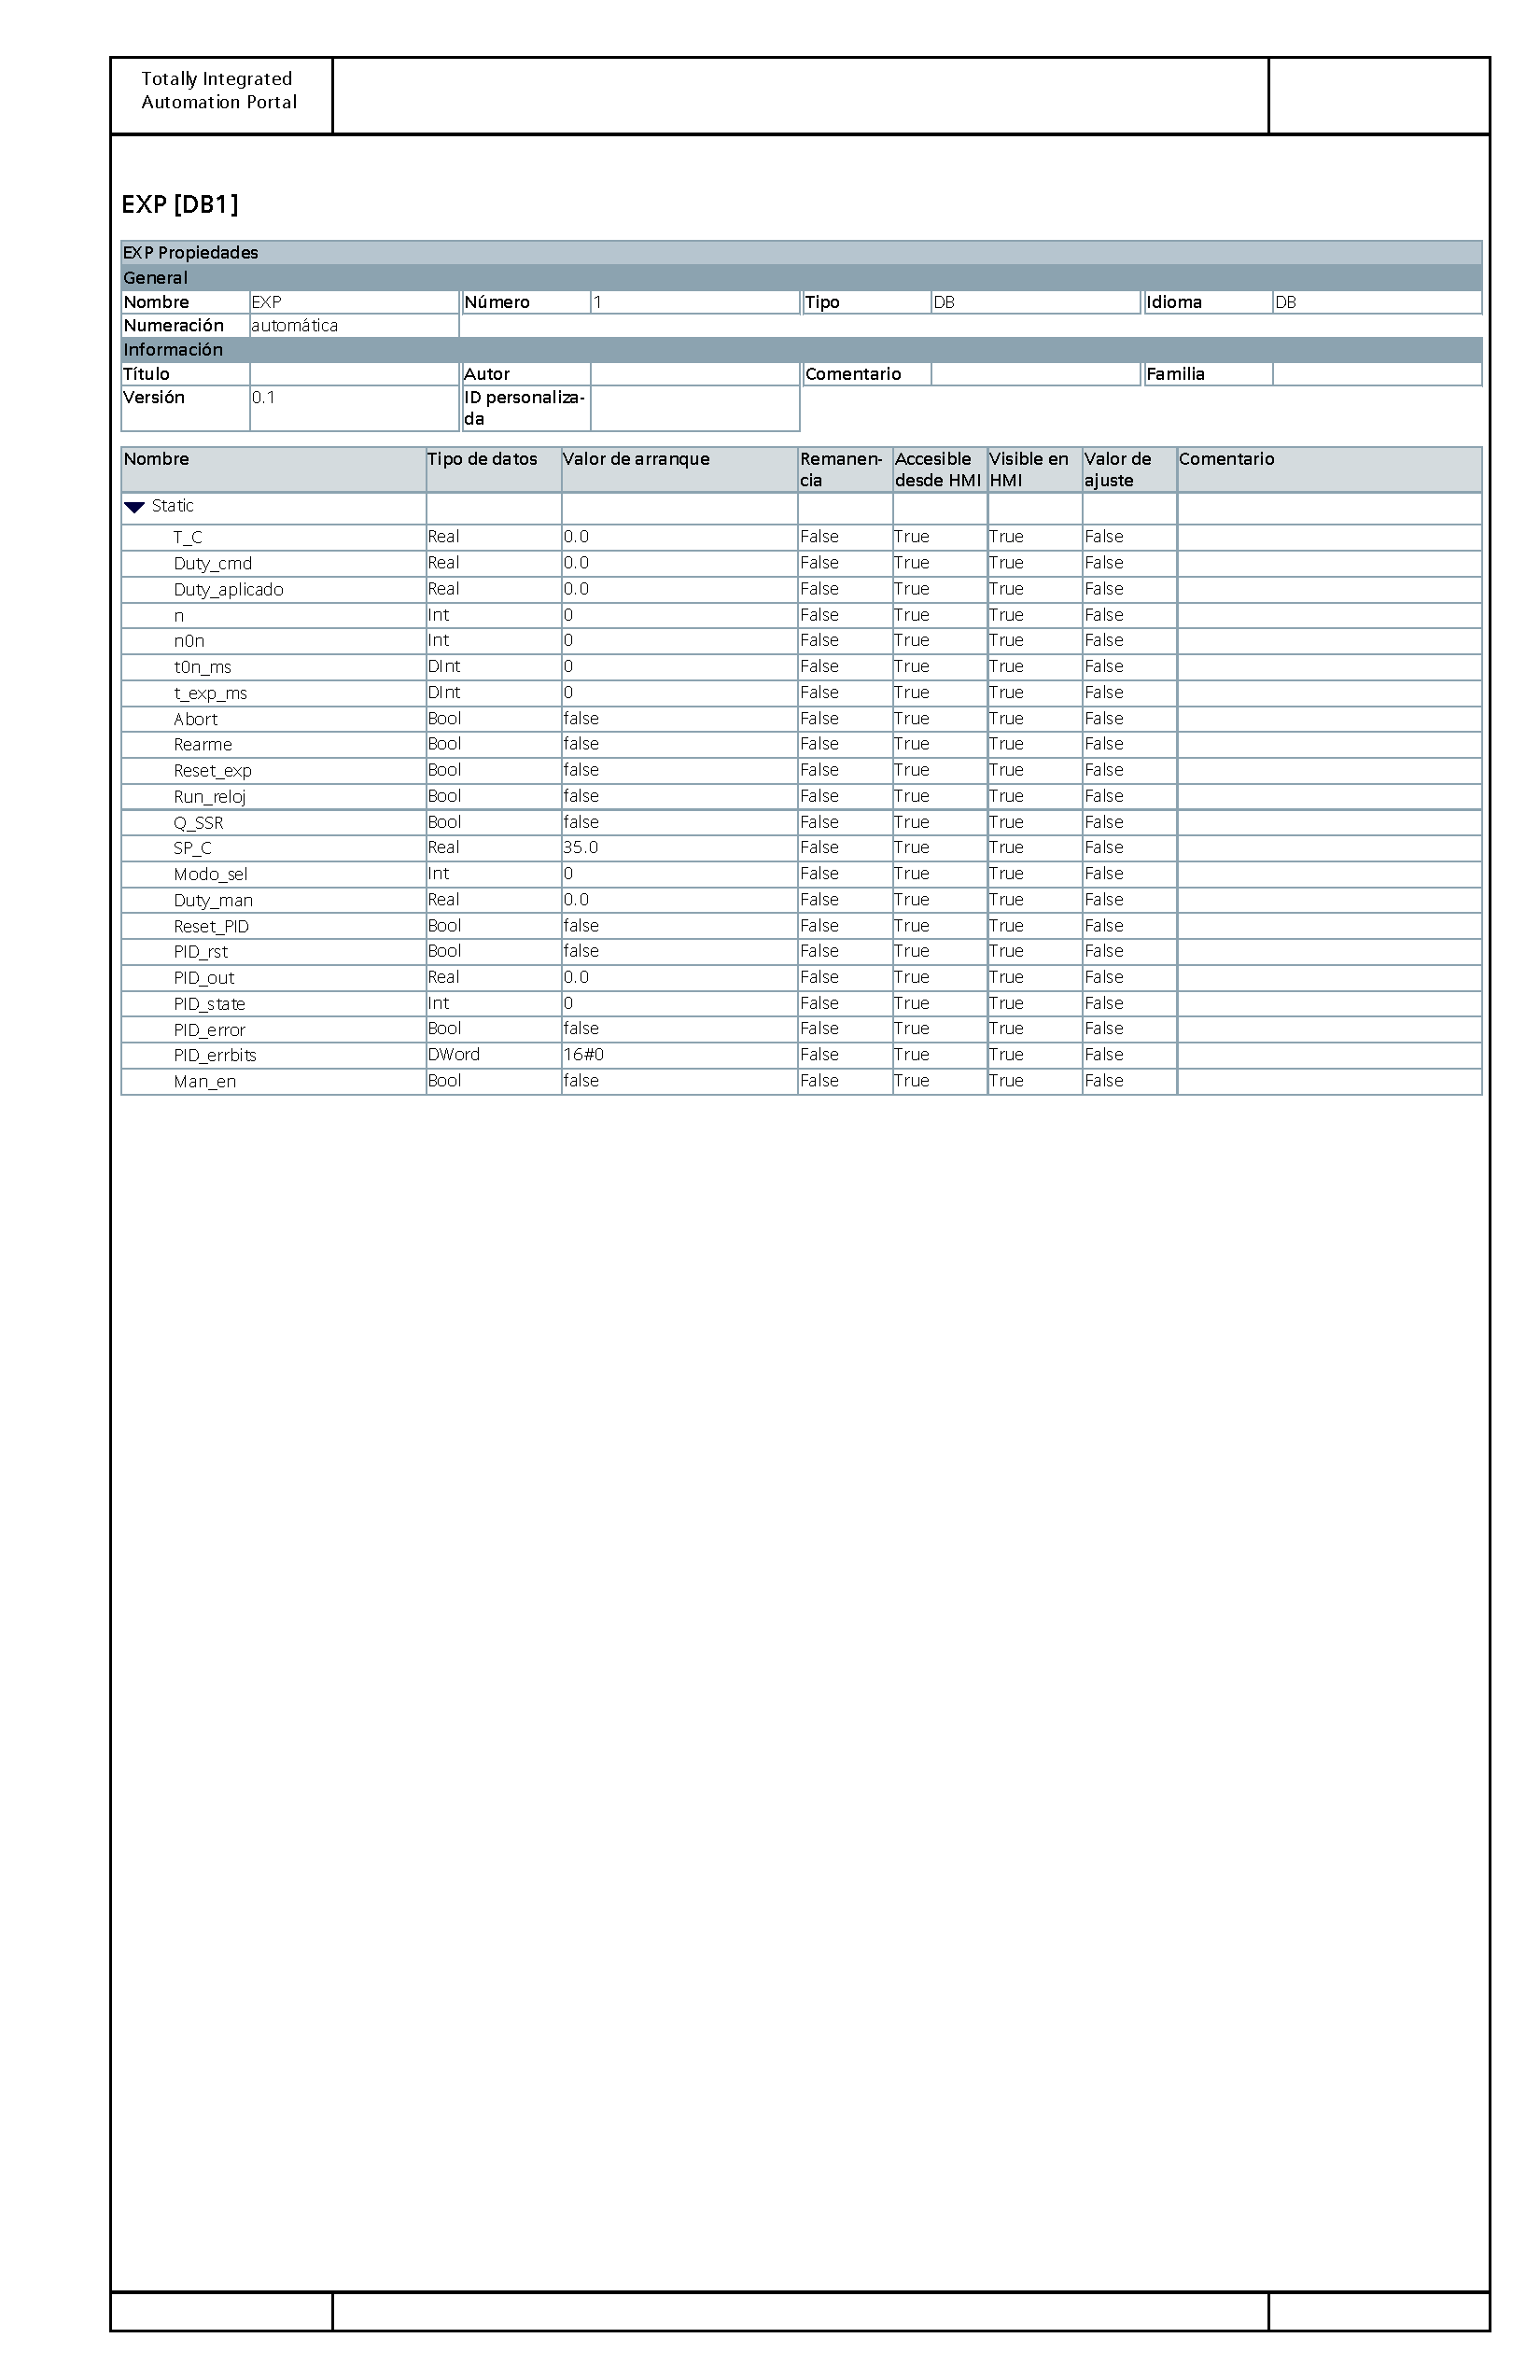
\includepdf[pages=1,scale=0.8,offset=0 -0.7cm,pagecommand={\thispagestyle{fancy}\noindent\textbf{J.4 Bloque de datos EXP (DB1)}}]{anexos/programa_plc/control_DB1_EXP.pdf}
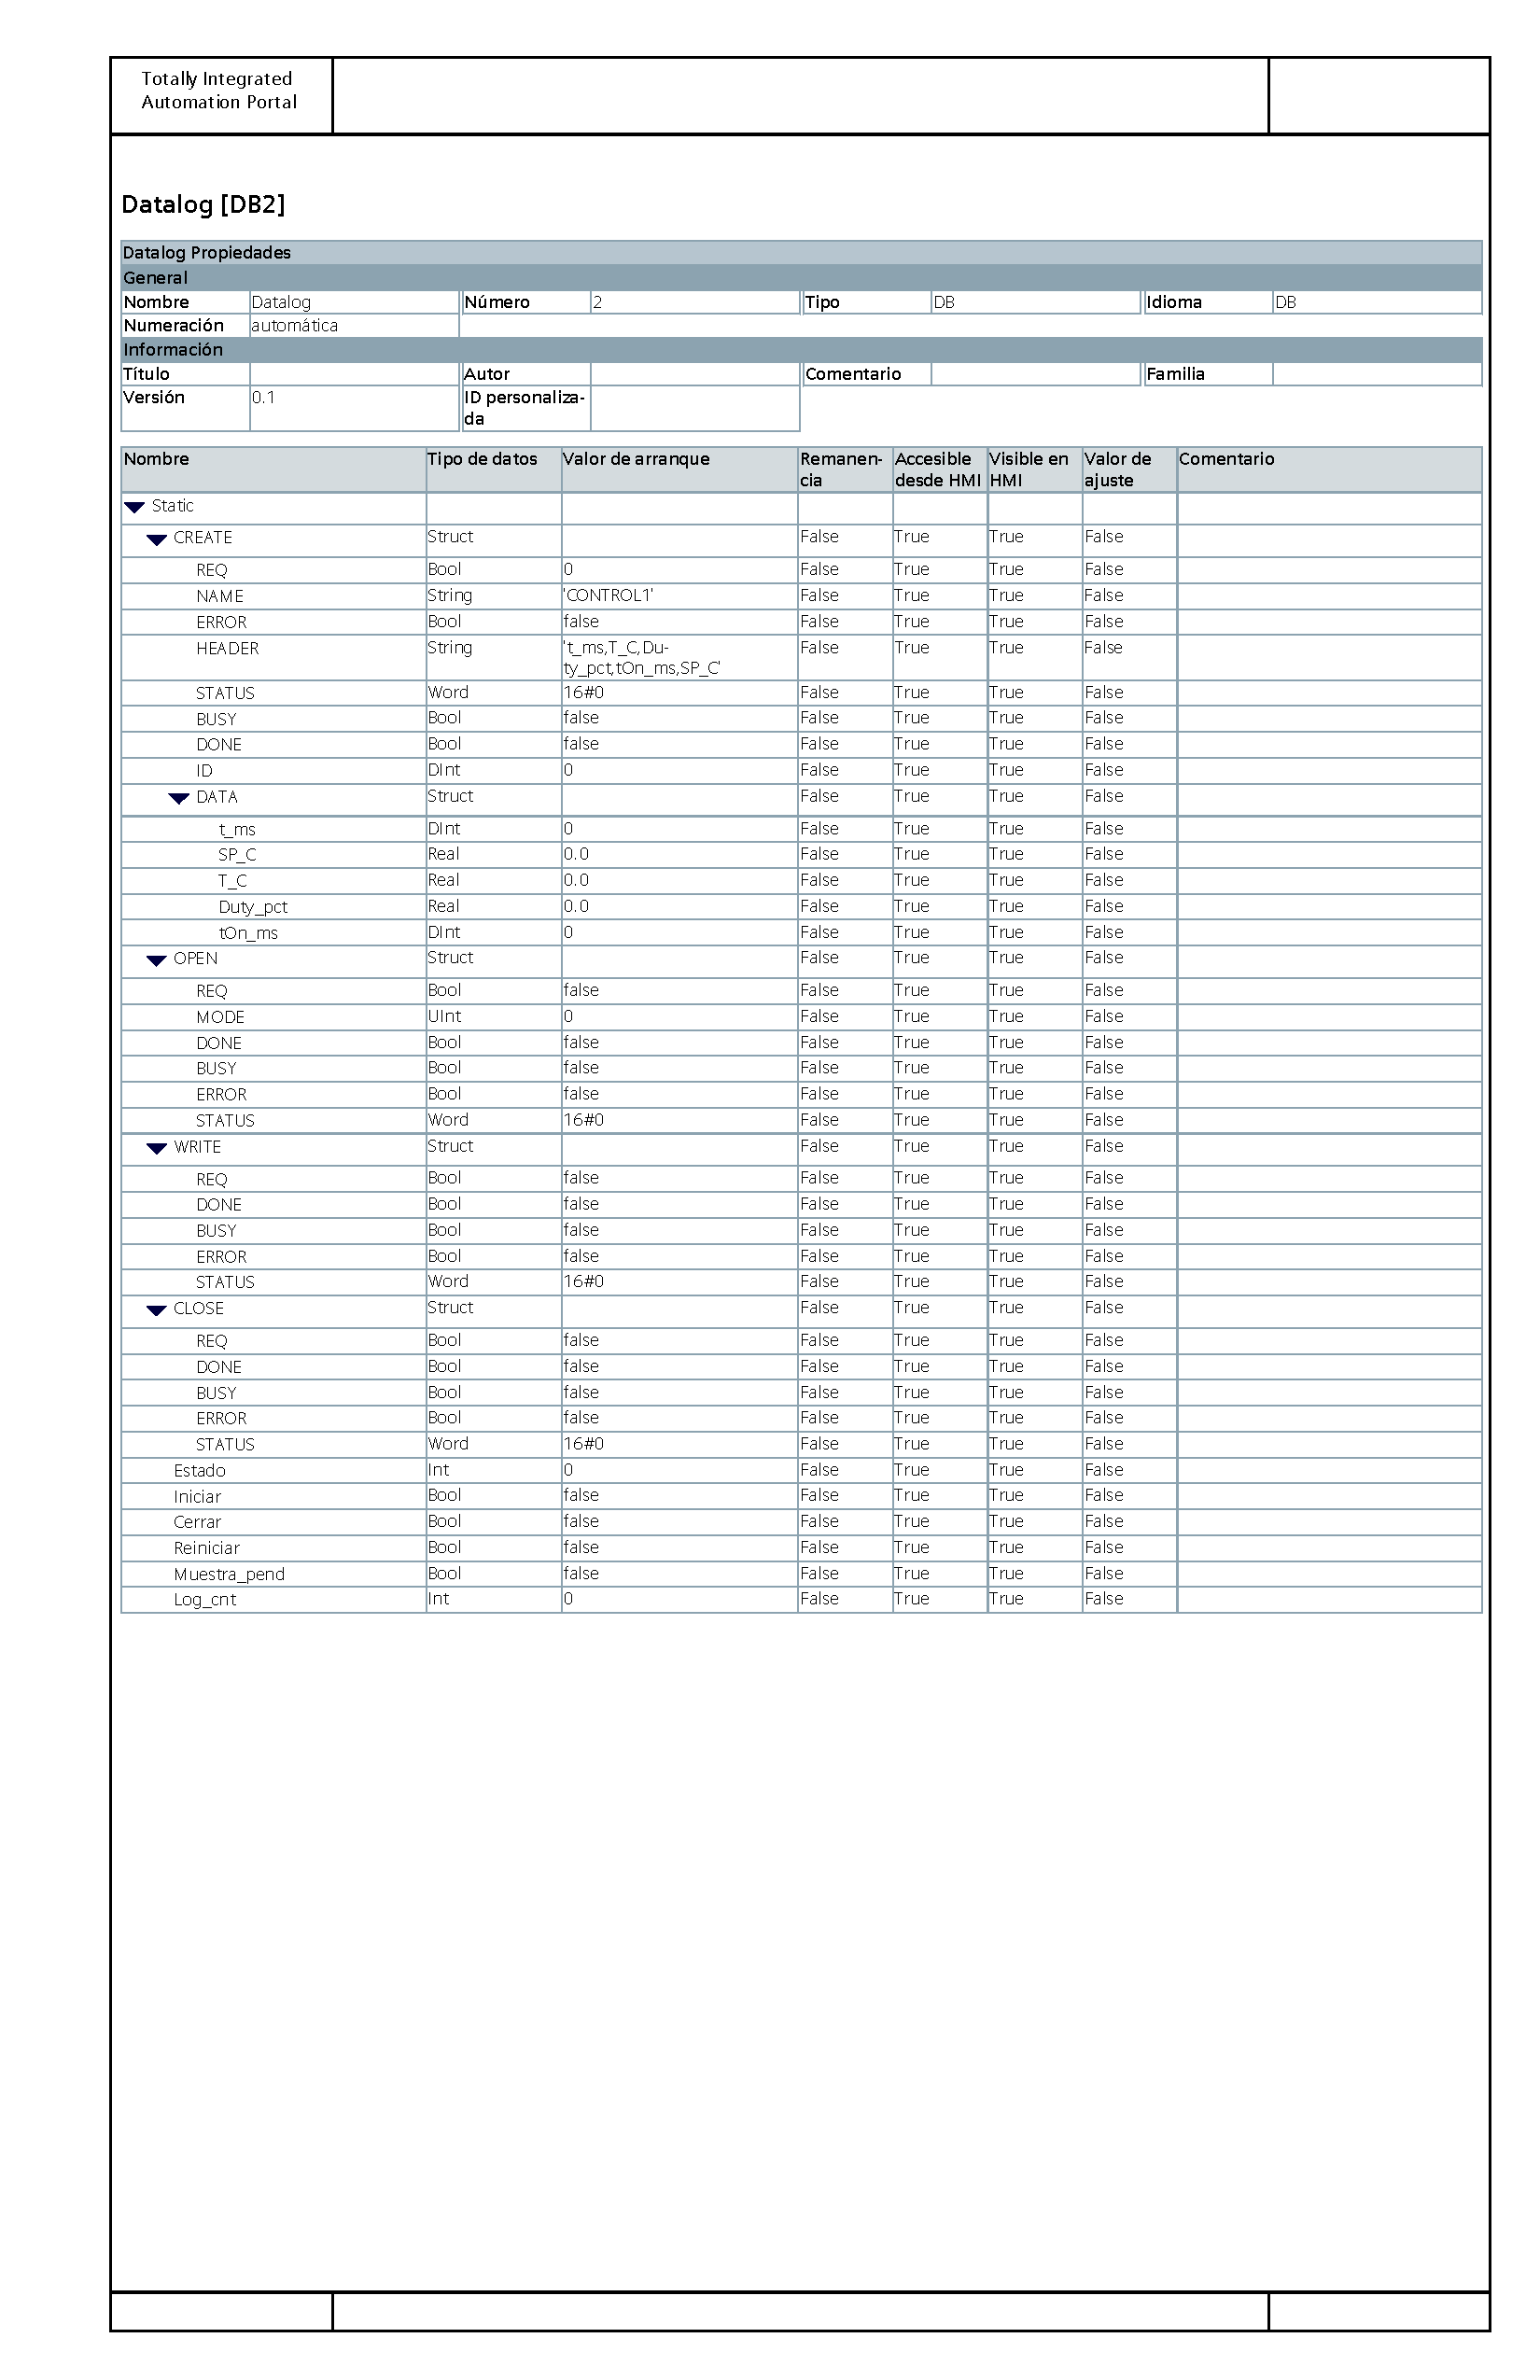
\includepdf[pages=1,scale=0.8,offset=0 -0.7cm,pagecommand={\thispagestyle{fancy}\noindent\textbf{J.5 Bloque de datos Datalog (DB2)}}]{anexos/programa_plc/control_DB2_Datalog.pdf}
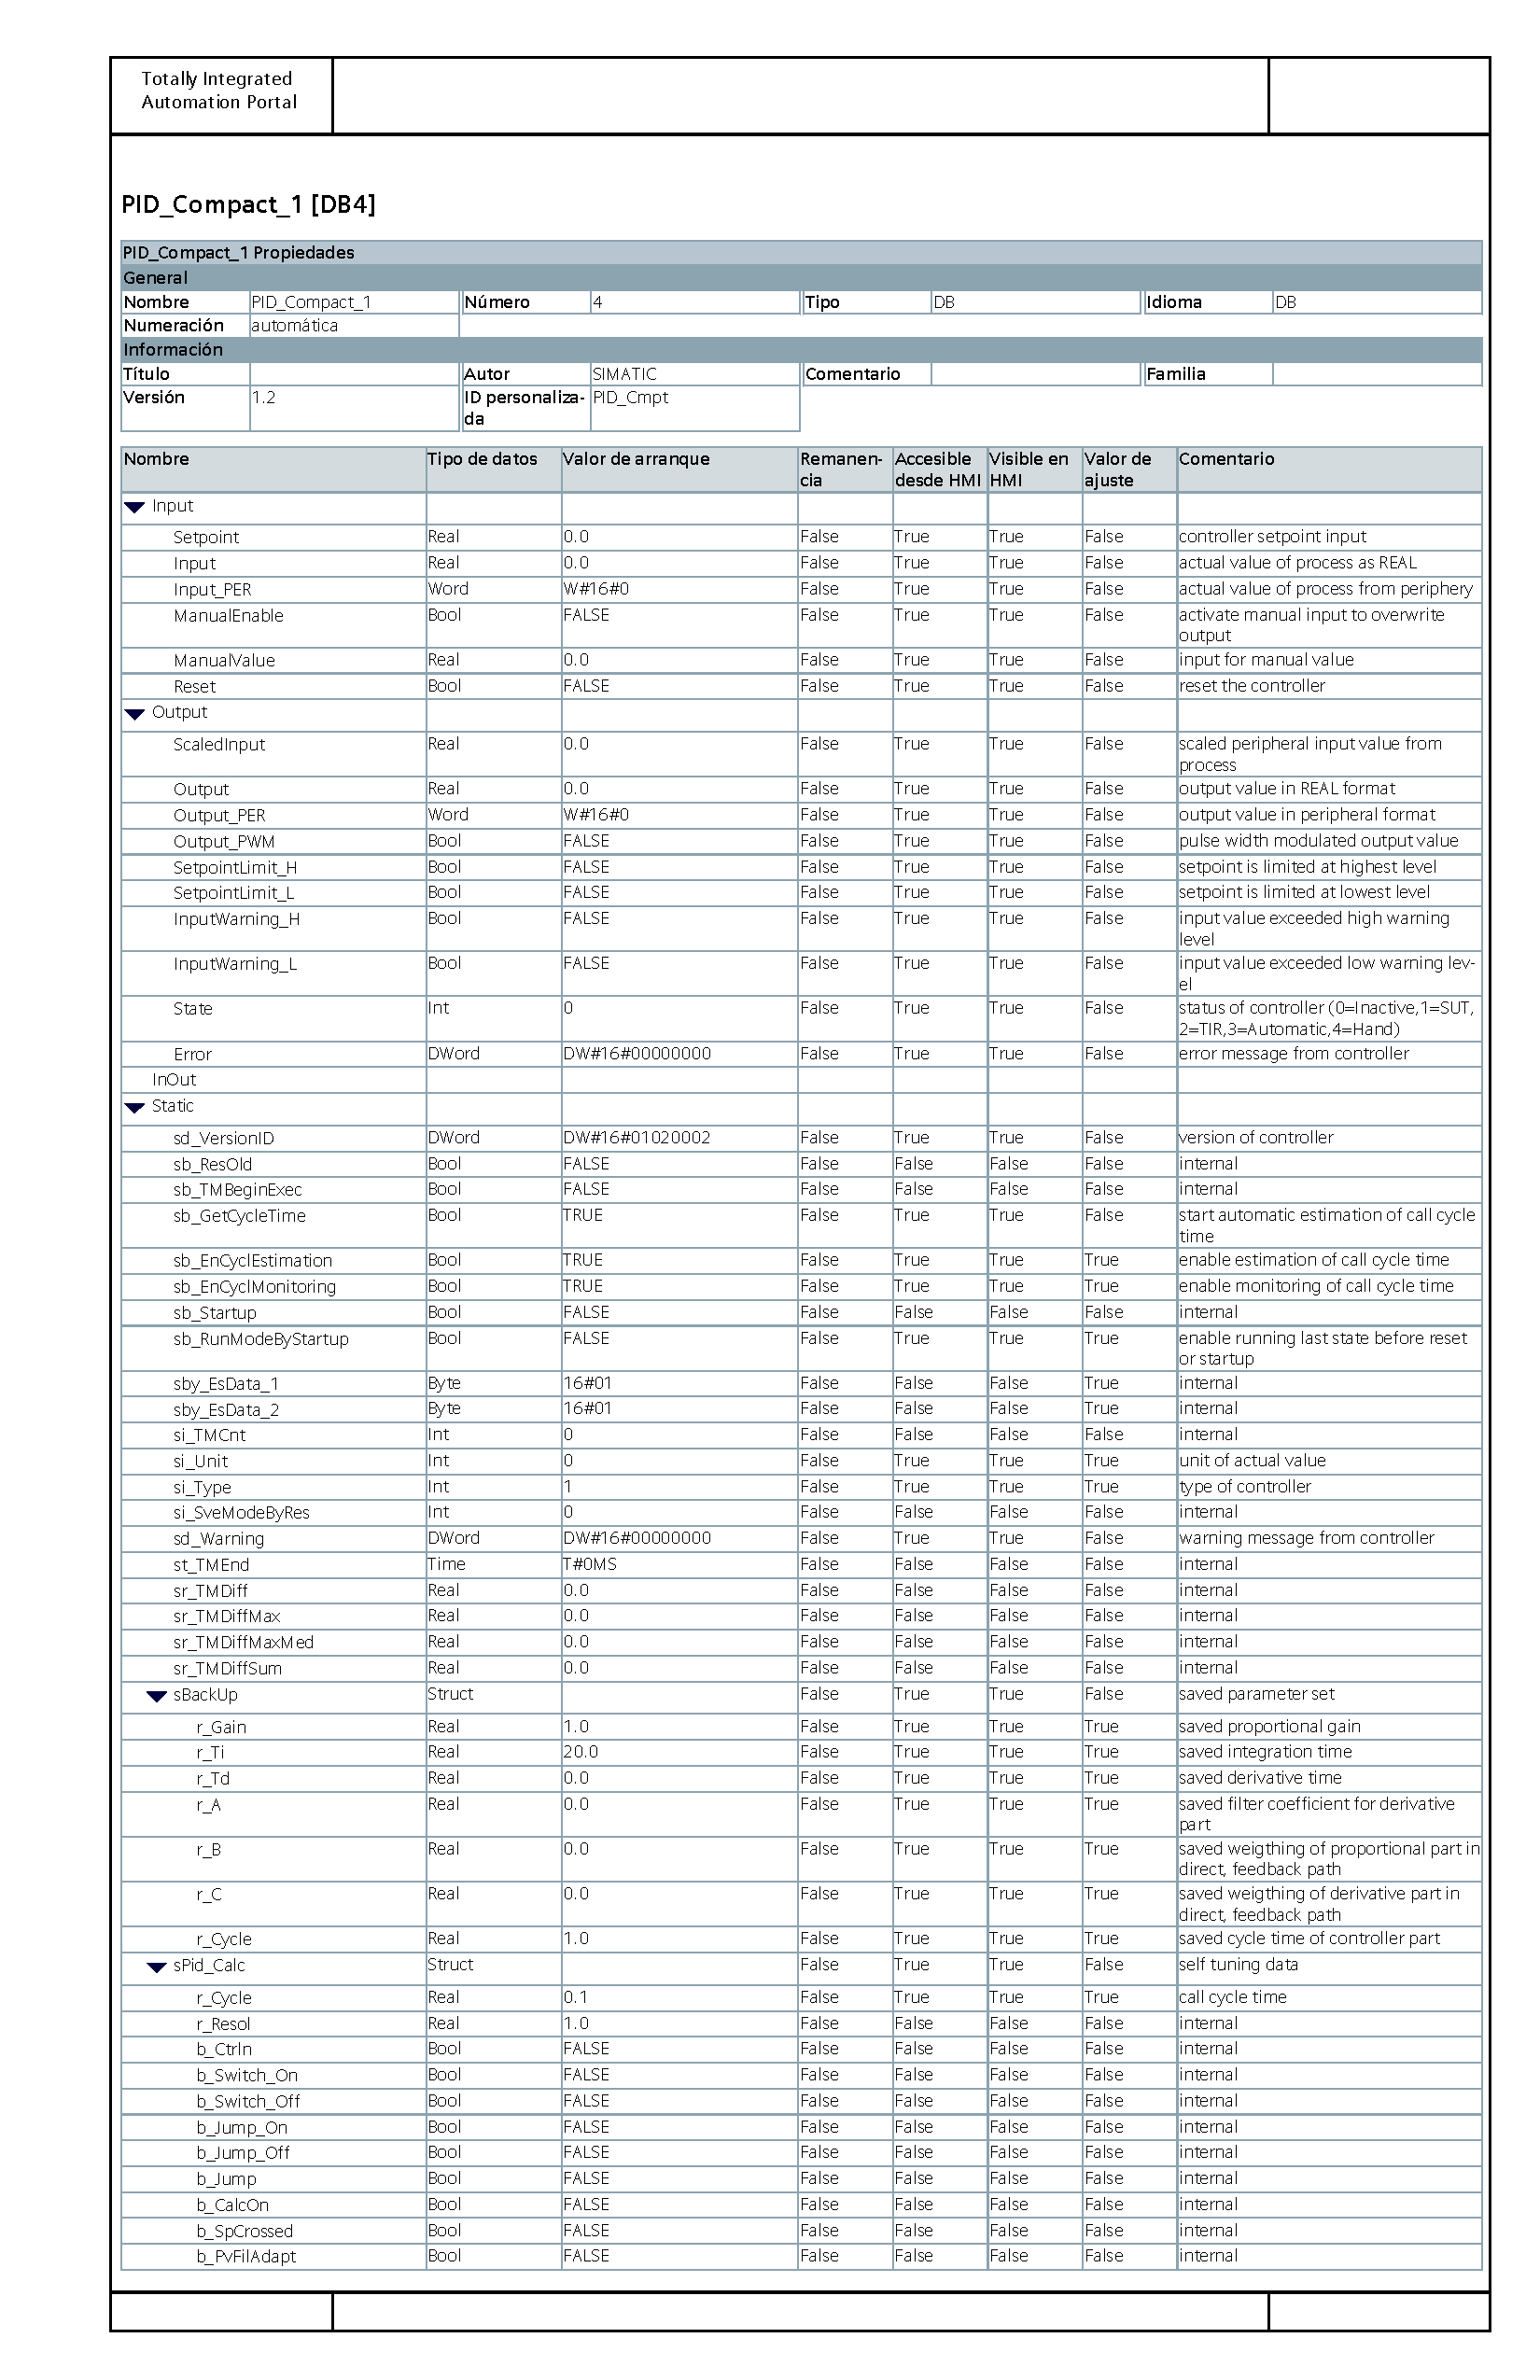
\includepdf[pages=1,scale=0.8,offset=0 -0.7cm,pagecommand={\thispagestyle{fancy}\noindent\textbf{J.6 Configuración del controlador PID\_Compact\_1 (DB4)}}]{anexos/programa_plc/control_DB4_PID_Compact.pdf}
\includepdf[pages=2-,scale=0.8,offset=0 -0.7cm,pagecommand={\thispagestyle{fancy}}]{anexos/programa_plc/control_DB4_PID_Compact.pdf}
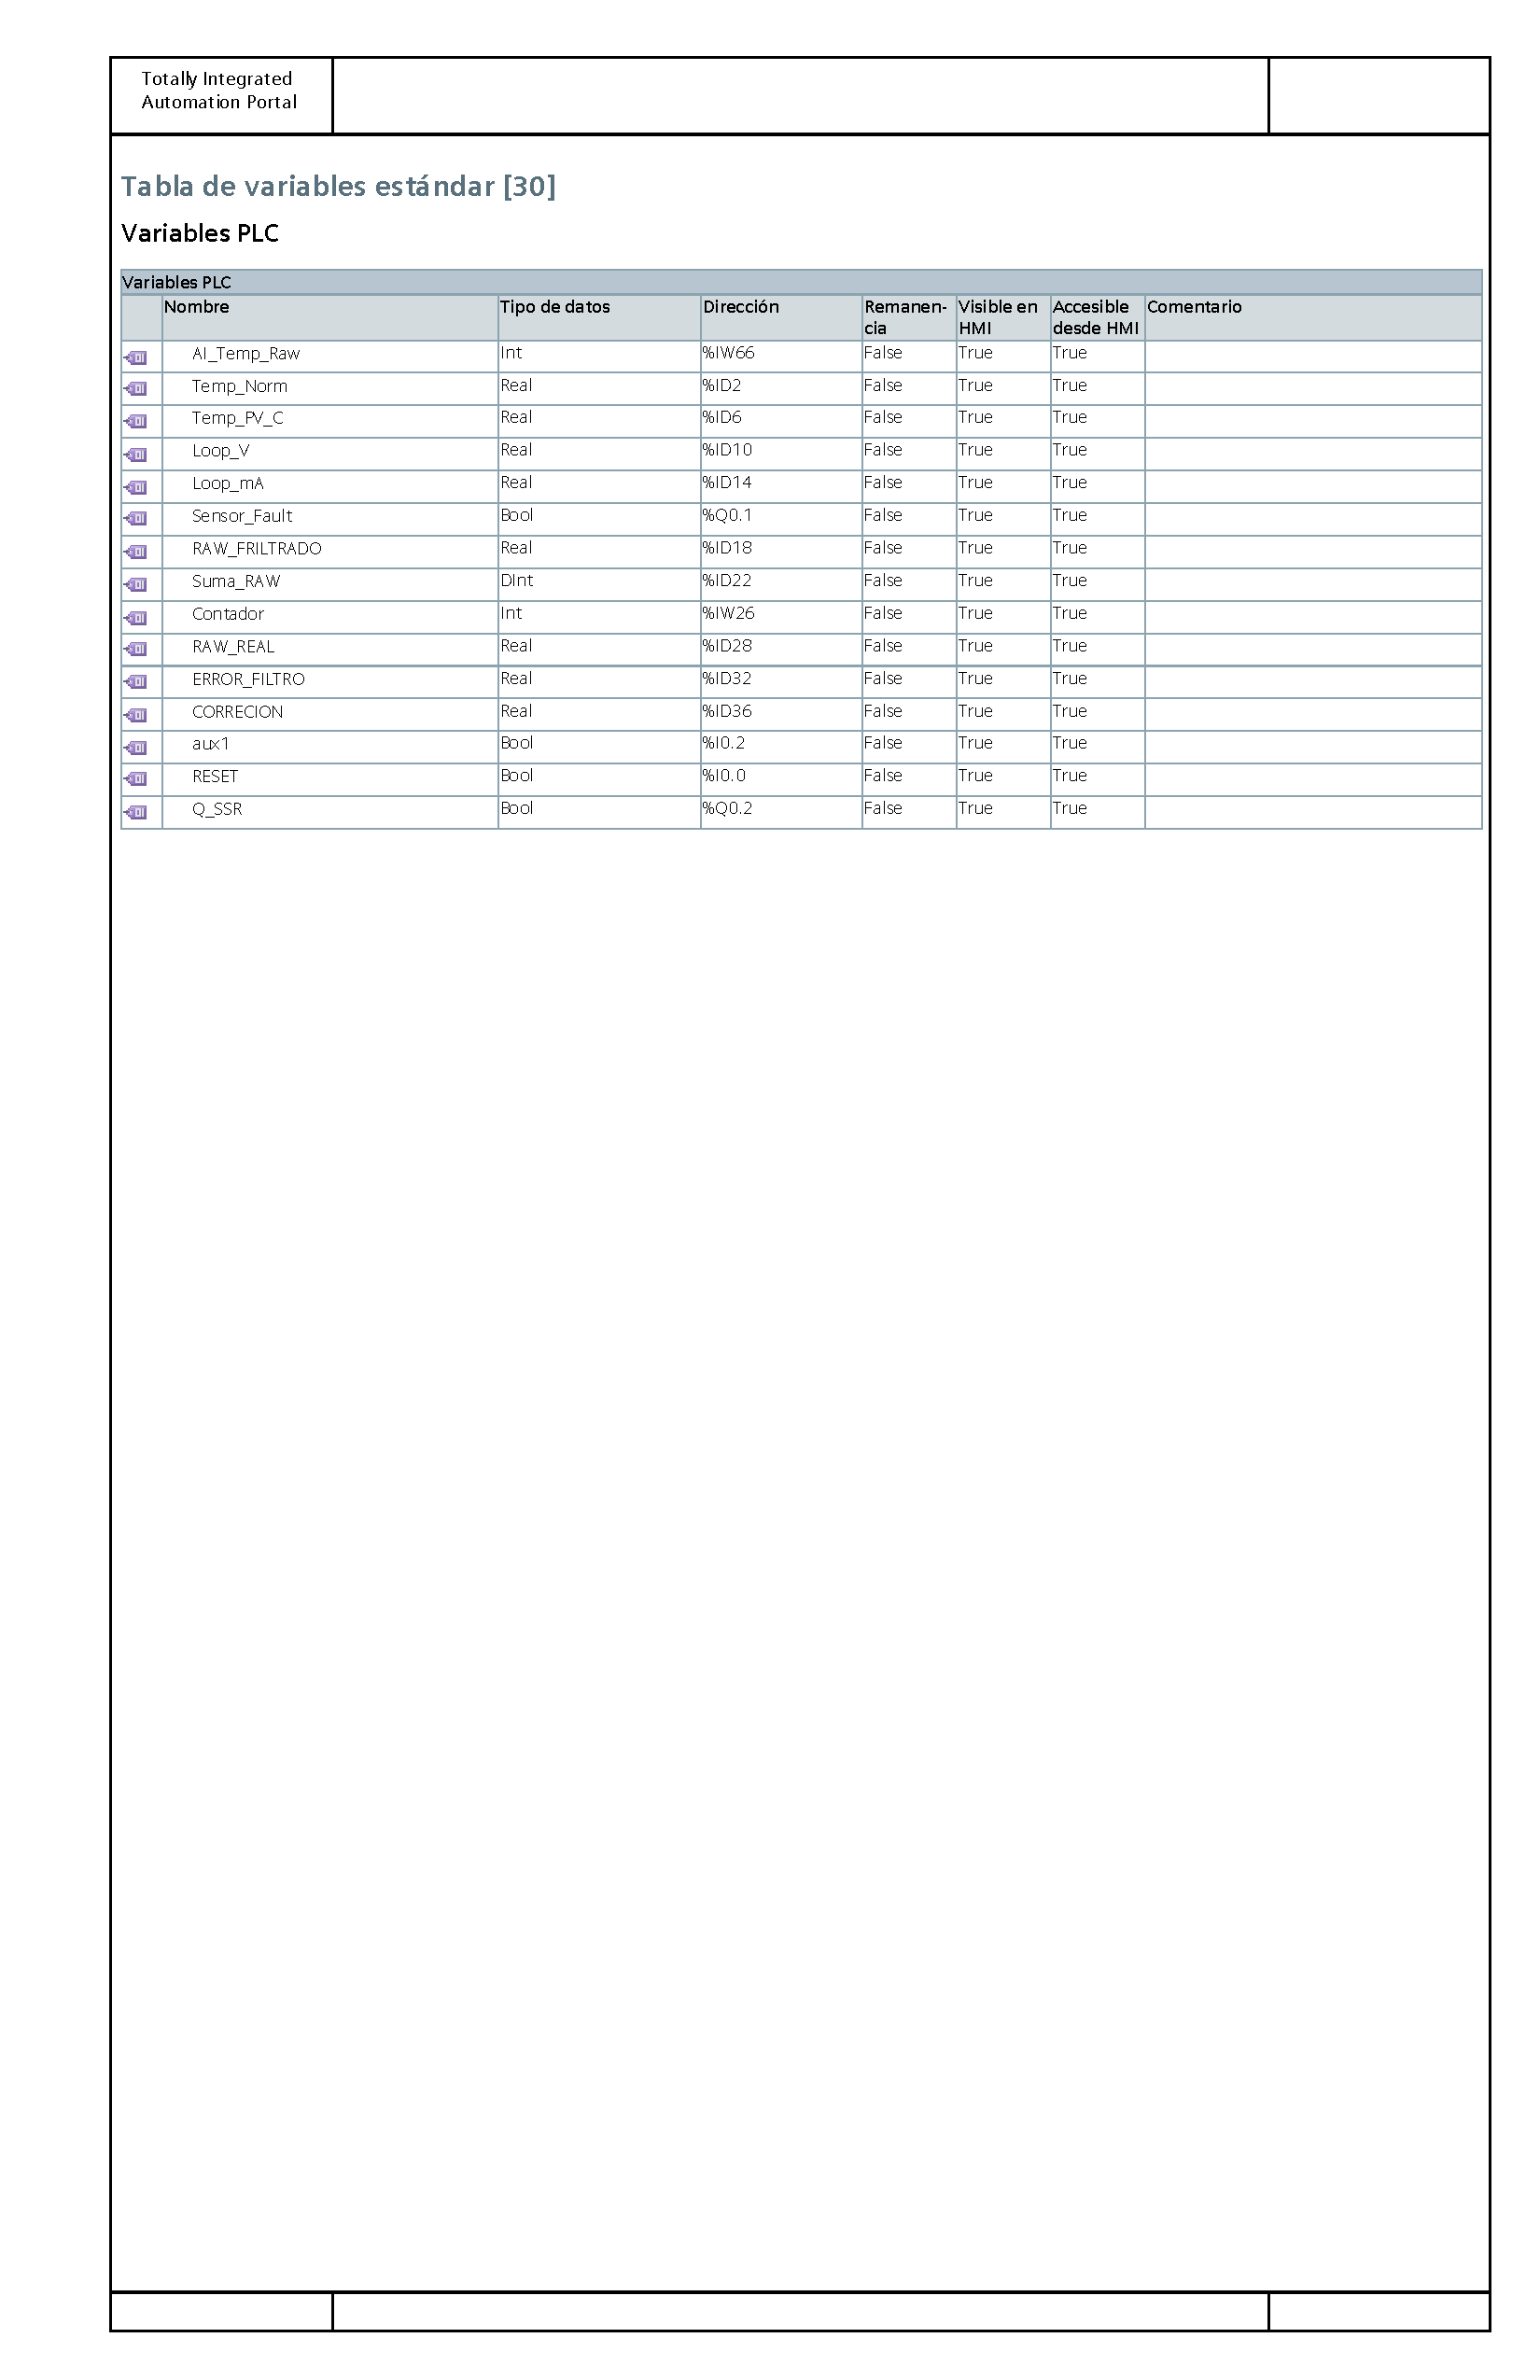
\includepdf[pages=1,scale=0.8,offset=0 -0.7cm,pagecommand={\thispagestyle{fancy}\noindent\textbf{J.7 Tabla de variables del PLC (programa de control)}}]{anexos/programa_plc/control_variables_plc.pdf}
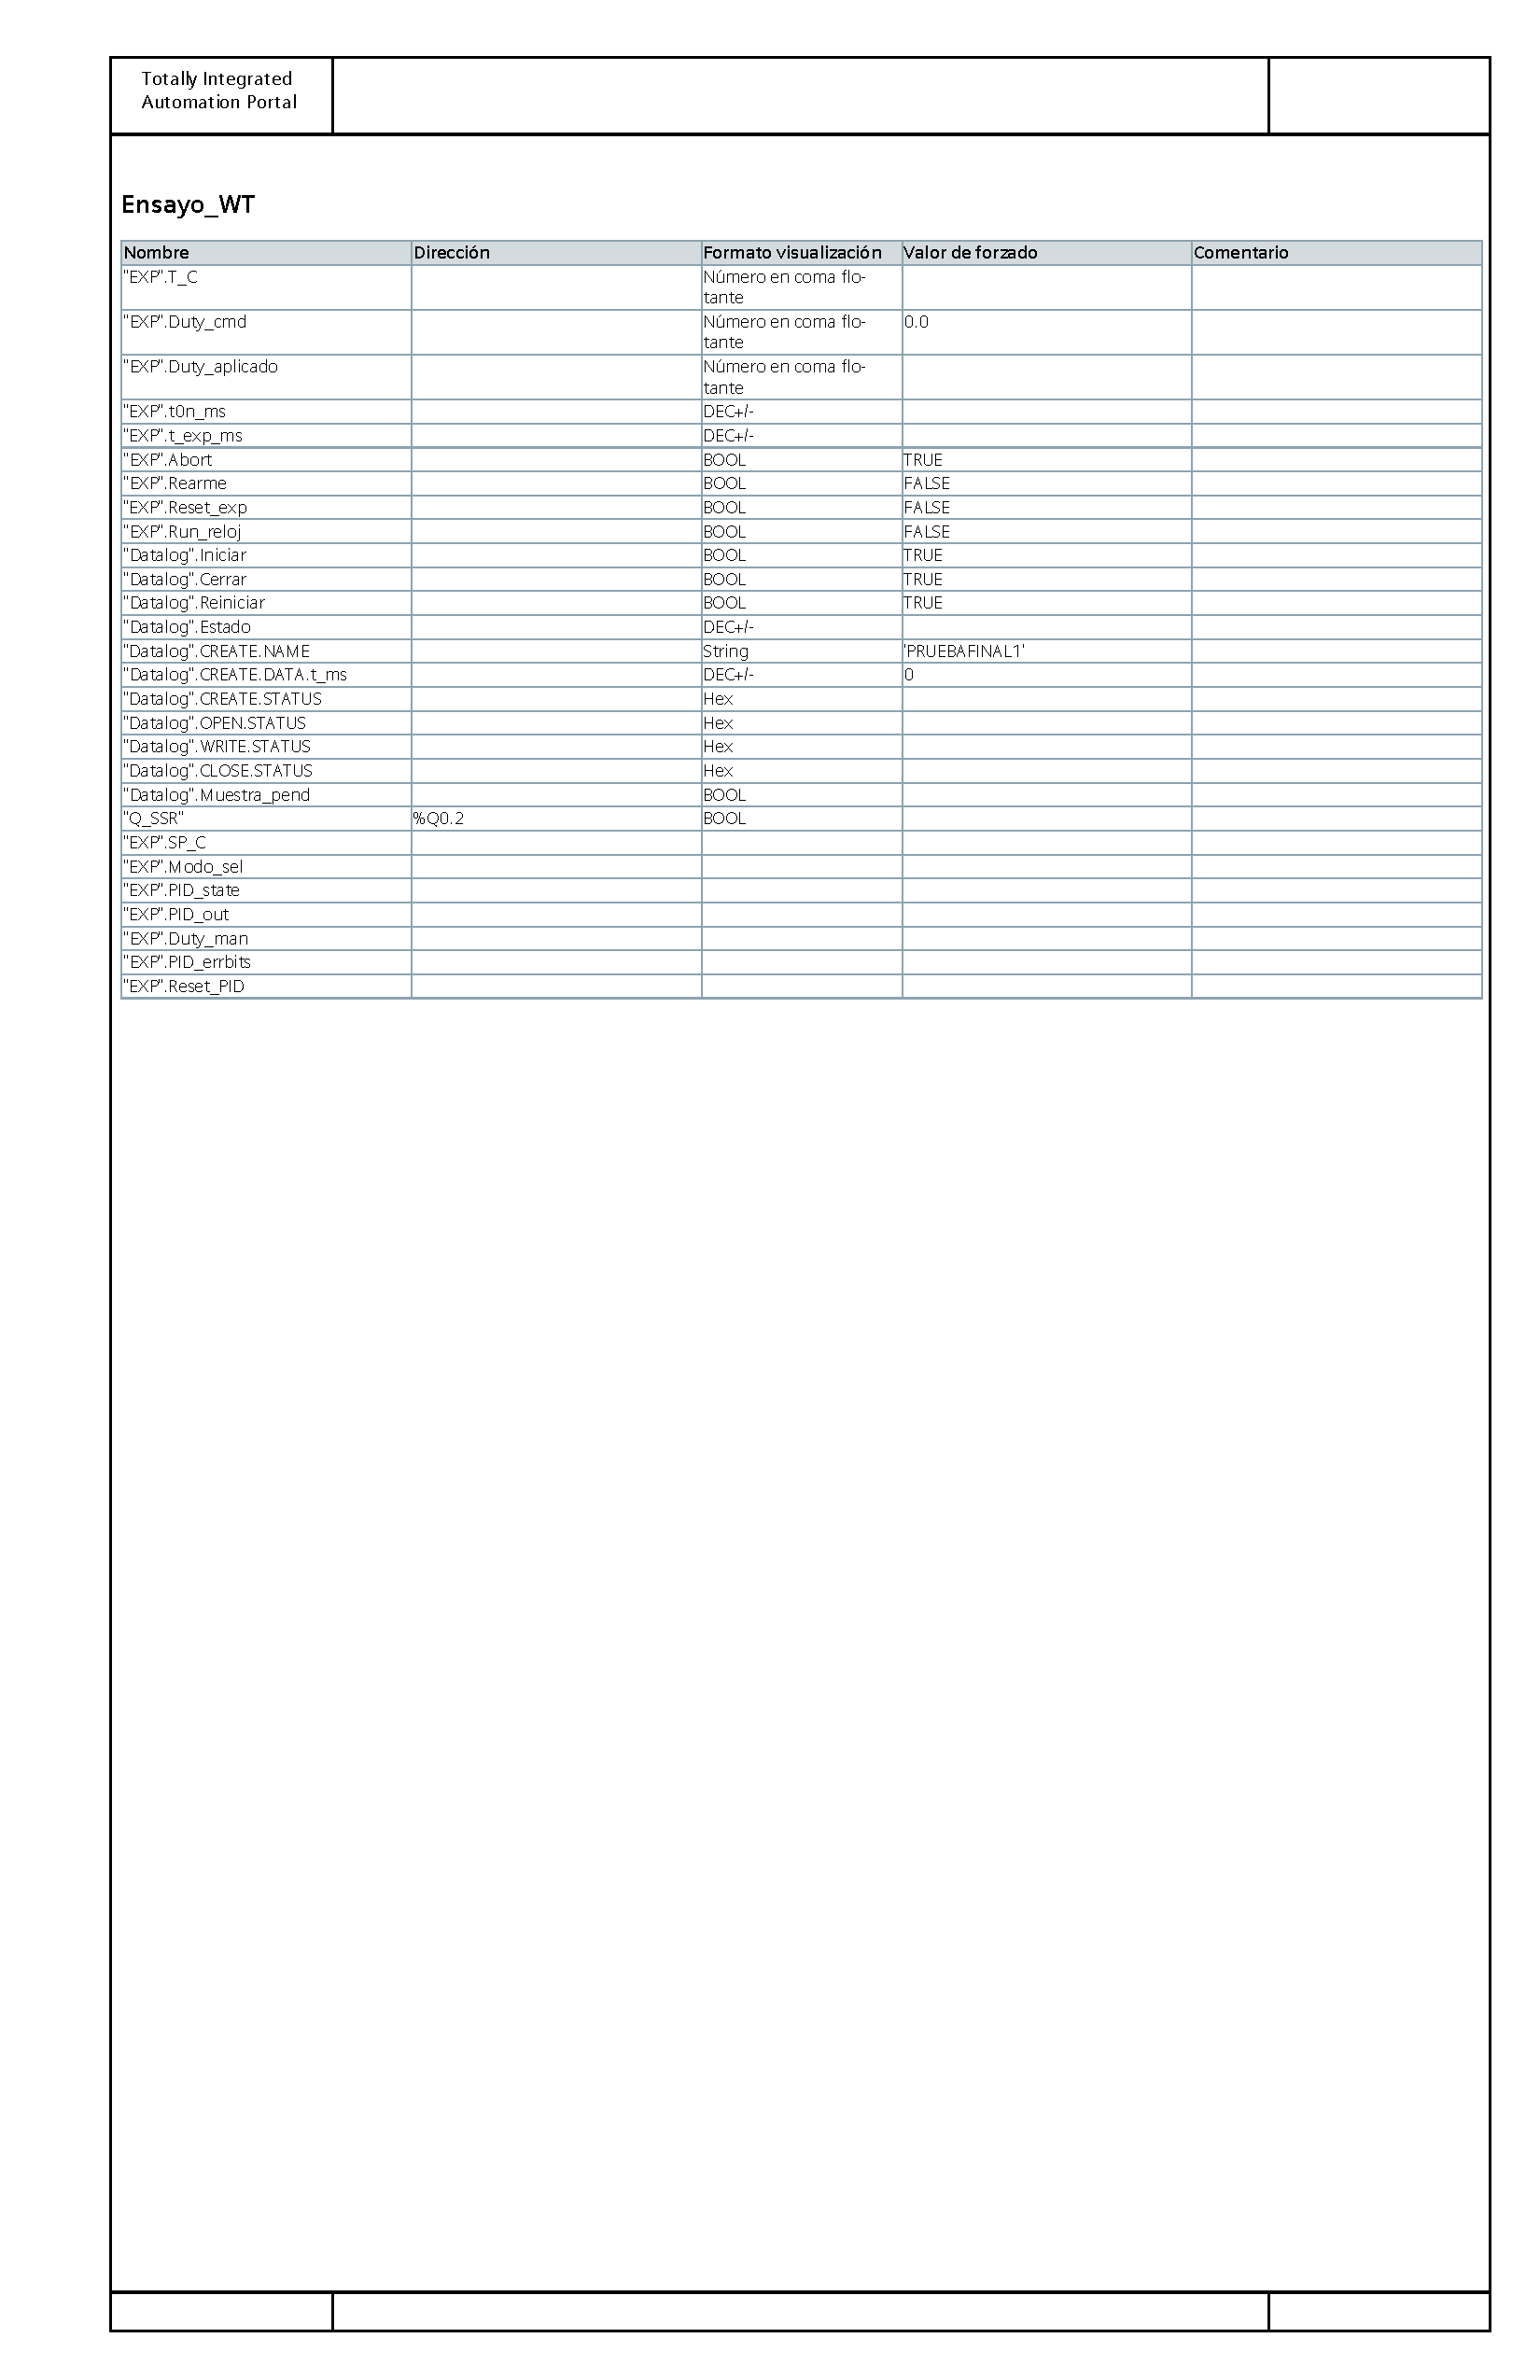
\includepdf[pages=1,scale=0.8,offset=0 -0.7cm,pagecommand={\thispagestyle{fancy}\noindent\textbf{J.8 Tabla de observación del ensayo}}]{anexos/programa_plc/control_tabla_observacion_ensayo.pdf}
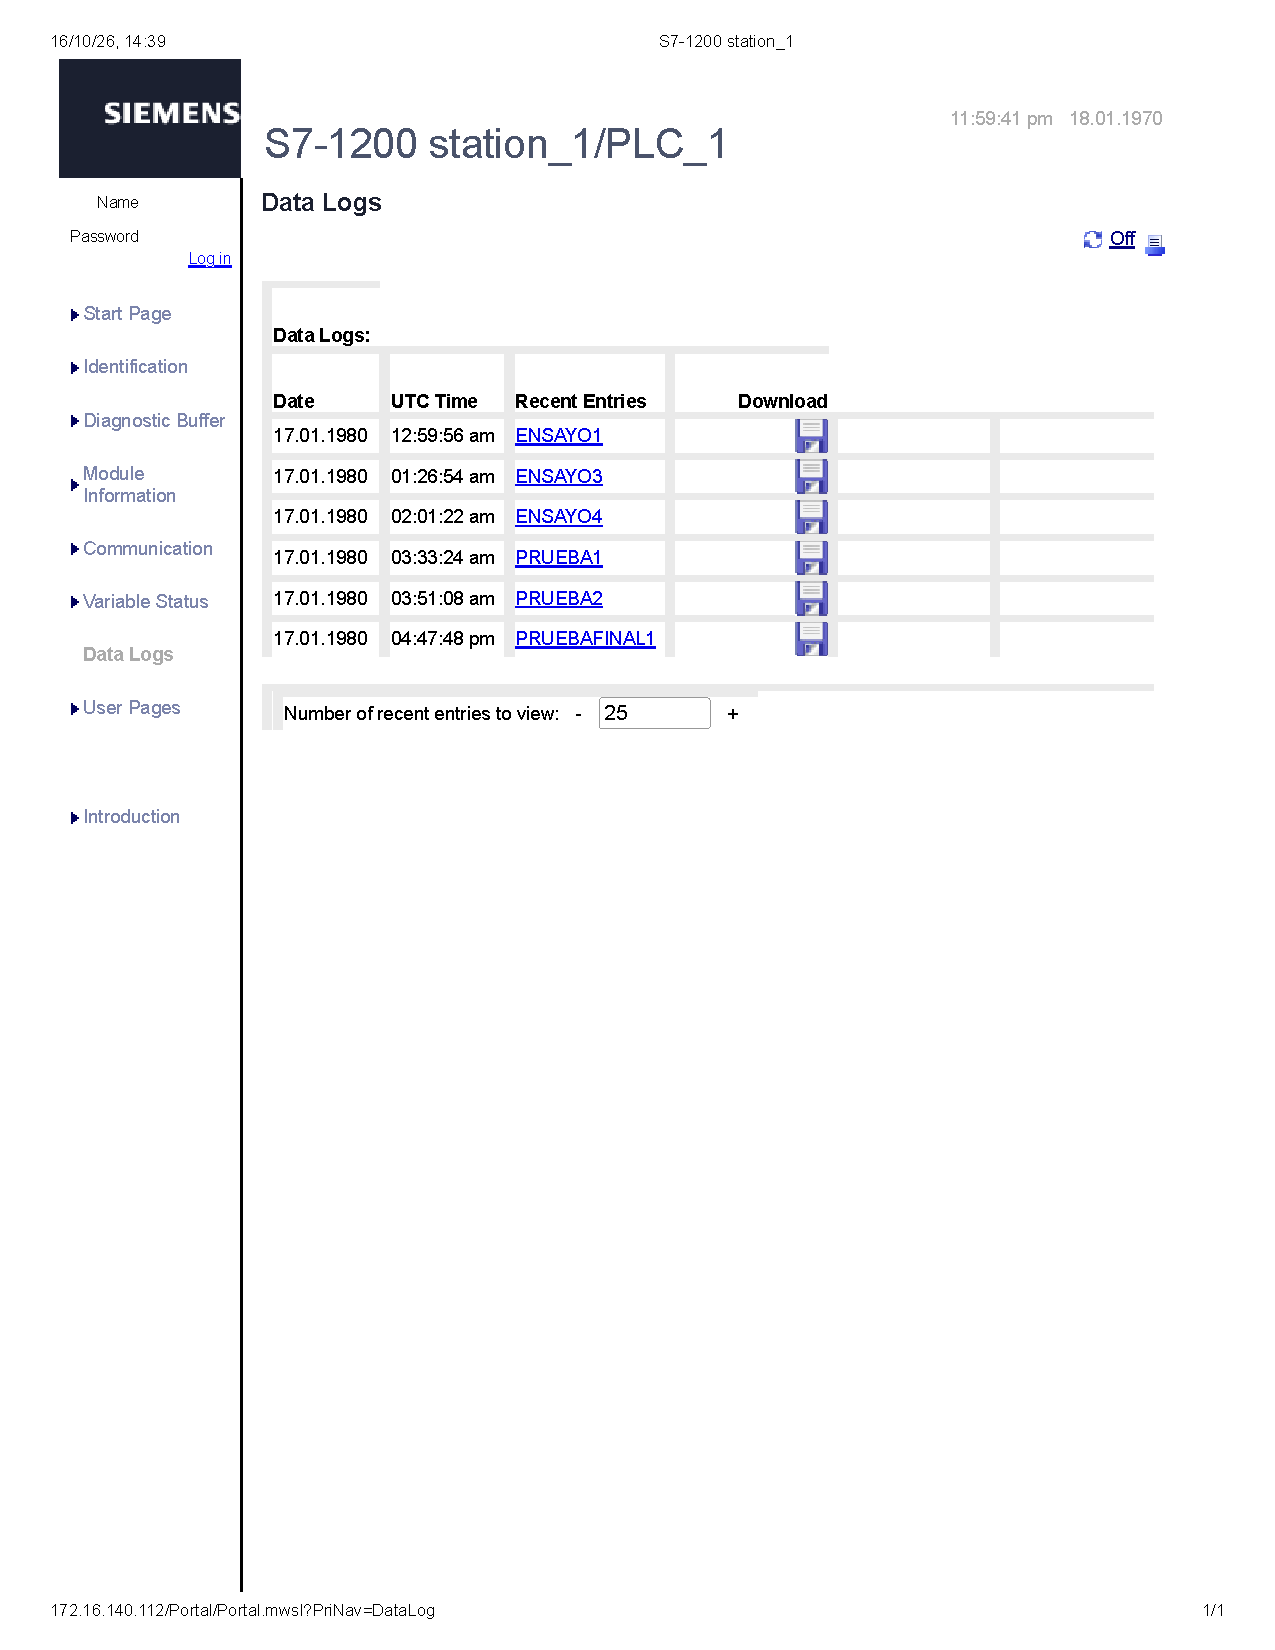
\includepdf[pages=1,scale=0.8,offset=0 -0.7cm,pagecommand={\thispagestyle{fancy}\noindent\textbf{J.9 Registros del servidor web del PLC (Data logs)}}]{anexos/programa_plc/servidor_web_data_logs.pdf}